\documentclass{article}
\usepackage[UTF8]{ctex}
\usepackage{geometry}
\usepackage{natbib}
\geometry{left=3.18cm,right=3.18cm,top=2.54cm,bottom=2.54cm}
\usepackage{graphicx}
\pagestyle{plain}	
\usepackage{setspace}
\usepackage{caption2}
\usepackage{datetime} %日期
\renewcommand{\today}{\number\year 年 \number\month 月 \number\day 日}
\renewcommand{\captionlabelfont}{\small}
\renewcommand{\captionfont}{\small}
\begin{document}

\begin{figure}
    \centering
    
\includegraphics[width=8cm]{upc.png}

    \label{figupc}
\end{figure}

	\begin{center}
		\quad \\
		\quad \\
		\heiti \fontsize{45}{17} \quad \quad \quad 
		\vskip 1.5cm
		\heiti \zihao{2} 《计算科学导论》课程总结报告
	\end{center}
	\vskip 2.0cm
		
	\begin{quotation}
% 	\begin{center}
		\doublespacing
		
        \zihao{4}\par\setlength\parindent{7em}
		\quad 

		学生姓名:\underline{\qquad  张一帆 \qquad \qquad}

		学\hspace{0.61cm} 号:\underline{\qquad 1907010214\qquad}
		
		专业班级:\underline{\qquad 本研人工智能 \qquad  }
		
        学\hspace{0.61cm} 院:\underline{计算机科学与技术学院}
% 	\end{center}
		\vskip 2cm
		\centering
		\begin{table}[h]
            \centering 
            \zihao{4}
            \begin{tabular}{|c|c|c|c|c|c|c|}
            % 这里的rl 与表格对应可以看到,姓名是r,右对齐的;学号是l,左对齐的;若想居中,使用c关键字。
                \hline
                课程认识 & 问题思 考 & 格式规范  & IT工具  & Latex附加  & 总分 & 评阅教师 \\
                30\% & 30\% & 20\% & 20\% & 10\% &  &  \\
                \hline
                 & & & & & &\\
                & & & & & &\\
                \hline
            \end{tabular}
        \end{table}
		\vskip 2cm
		\today
	\end{quotation}

\thispagestyle{empty}
\newpage
\setcounter{page}{1}
% 在这之前是封面,在这之后是正文
\section{引言}
进入大学,是我们从小一直以来学习的目标,但是,大学并不是个游戏的天堂,而是个挥洒汗水为理想繁多蓬勃的地方。光阴似箭,属于我的大学的第一个学期已经快结束了,而经过一个学期对计算科学导论这门课程的学习,我对计算机已经有了初步的了解。下面我就来浅谈一下我对计算科学导论这门课程的理解。

【关键字】:计算科学;计算机;发展;总结

\section{对计算科学导论这门课程的认识、体会}


\subsection{什么是计算机?}
计算机(computer)俗称电脑,是现代一种用于高速计算的电子计算机器,可以进行数值计算,又可以进行逻辑计算,还具有存储记忆功能。是能够按照程序运行,自动、高速处理海量数据的现代化智能电子设备。由硬件系统和软件系统所组成,没有安装任何软件的计算机称为裸机。可分为超级计算机、工业控制计算机、网络计算机、个人计算机、嵌入式计算机五类,较先进的计算机有生物计算机、光子计算机、量子计算机等。计算机的基本能力是有限的、简单的,但能够通过程序将其组合成复杂的、强大的能力。其他技术的发展,特别是半导体技术和激光技术推动了计算机的更新换代,价格越来越低,能力却越来越强。



\begin{table}[!htbp]
    \centering
    \renewcommand{\arraystretch}{2}
\begin{tabular}{|c|c|}
% 这里的rl 与表格对应可以看到,姓名是r,右对齐的;学号是l,左对齐的;若想居中,使用c关键字。
    \hline
    第一代(1945-1957): &电子管计算机 \\
    \hline
    第二代(1958-1963): & 晶体管计算机 \\ \hline
    第三代(1964-1969): & 小规模集成电路计算机 \\ \hline
    第四代(1970-1990): & 以微处理器为标志的大规模集成电路计算机\\ 
    \hline
    第五代(1991-至今): & 以互联网为标志的信息系统\\ \hline
\end{tabular}
    \label{table1}\caption{计算机的更新换代}
\end{table}

\subsection{计算机的发展}
世界上最古老的计算机应该是算盘这样的简单计算工具。随着社会的发展和科技的进步,有许多人为计算机的功能进步起了重要作用,其中,影响最大的莫过于被称为“现代计算机之父”的冯·诺依曼教授。他对计算机概念的描述影响了计算机的发展方向,使它最终发展成现在我们所见到的样子,使它越来越多样化,并逐步深入到我们的生活和工作中。
\subsection{计算科学一词的来历}
最令我印象深刻的莫过于前几节课了,但是孙老师以生动有趣的授课方式告诉了我们什么是计算科学,让我受益良多。我通过阅读《计算科学导论》\cite{ref1}这本书,知道了从20世纪30年代到60年代初,计算机科学与技术的研究与学科发展基本上处在萌芽状态,当时从事计算机科学与技术研究的科学家主要来自数学和电子科学领域。20世纪50年代后期高级程序设计语言的发展促进了硬件、软件与理论的融合,计算的数学理论、通用电子数字计算机系统、科学计算、高级语言程序设计等多个方向的研究进展催生了计算机科学作为一个学科的出现。而经过我通读了课本第一章,知道曾经有人提出过这样一个问题:计算科学能否作为一门学科呢?我倒是觉得,计算科学作为一门学科完全没有问题,有关计算科学定义,研究对象,研究范畴以及读者将要看到的学科的来龙去脉和学科的内涵都将有力地从正面回答这个问题。但是,通过我搜素百度得知\cite{ref2}计算科学一词却包含着两方面的内涵,有狭义和广义之分。狭义的计算科学指称的就是我的专业——计算机科学与技术。其研究内容覆盖了对计算问题的一般研究。而广义的计算科学包含的内容要广得多,他不仅覆盖了计算机科学与技术的研究范畴,而且还包含更多的内涵。
\subsection{对导论这门课的理解与认识}
我认为计算科学导论是针对计算机科学初学者而开设的。通过阅读姜海涛的论文\cite{ref3}我得知计算科学导论这门课在一个大一新生对整个学科还缺乏深入,全面了解的情况下,从科学哲学理论的角度对计算机科学与技术的定义,范畴,特点,基本问题,发展主线,学科分类,知识组织结构,学科发展的特点和内在规律以及从事学科工作的基本工作流程建立起一种基本的,科学性的认识,对如何使自己富有创新意识,逐步成长为创新人才建立起一种基本的,正确的科学认识。它并不要求初学者广泛借阅图书资料,因为初学者并不具备同时掌握几个体系的能力与知识基础,并且很少涉及具体的,系统的专业知识,特别是操作使用计算机的技术知识,它仅是为初学者学习基础课程和后续计算机科学与技术课程的一个导引,培养学生们的兴趣,俗话说就是将同学们引进门。任何一门学科或专业,都含有丰富的人文内容和特质,都可以进行人文教育,使学生在学习中感受到美的熏陶与生命力量的提升,在计算科学导论的教学过程中,以一种什么样的意义来揭示该学科,就帮助学生设置一个学习的方向。方向不同,学生在从事学习过程中进行的心理活动不同,学习的结果也不同。对知识,学生会记忆性地学,对技能,学生会模仿性地学,对能力方面,学生会思维地学,对伦理方面,学生会体验地学。无论如何,教学过程中的引导作用是非常明显也是极其重要的。并且相信几乎占据导论“半壁江山”的学科意义,内容,方法,健康成长是任意一本专业书都不会出现的。也就是说,这门课是为了培养高素质的计算机科学与技术专业人才的一个导引。而且我们应该认识到,任何高校开设的任何学科都有其滞后性,在我们掌握了一门新技术同时会有更新的技术产生。而我们这一专业更为严重,更为突出,也许在校期间学习的东西在毕业后已经不适合用啦。正如我们现在学习的程序语言,也许在走出校门后又会出现新的语言。所以说,我们要学好这一学科的知识,更需要创新,提高自学能力和接受新事物的能力。因为我们这一学科本来就是走在时代前沿的一门学科,更需要紧跟时代的步伐。面对我们这一专业的机遇与挑战,我们既要对我们这一专业有美好的憧憬和希望,又要脚踏实地的学习,牢固掌握基础知识同时要多读一些与专业有关的书籍加深对所学知识的理解和应用,从而提高自己的能力。而计算科学导论,正是在为我们打下基础,它起到一个奠基的作用。只有在我们深刻理解计算机和计算科学的原理之后,才能适应日后日新月异的大环境,才能做出我们自己的创新成果。                                                                                                                                                 \section{进一步的思考}

\begin{itemize}
    \item 人工智能是计算机科学的一个分支,它企图了解智能的实质,并生产出一种新的能以人类智能相似的方式做出反应的智能机器,该领域的研究包括机器人、语言识别、图像识别、自然语言处理和专家系统等。人工智能从诞生以来,理论和技术日益成熟,应用领域也不断扩大,可以设想,未来人工智能带来的科技产品,将会是人类智慧的“容器”。人工智能可以对人的意识、思维的信息过程的模拟。人工智能不是人的智能,但能像人那样思考、也可能超过人的智能。人工智能也是一门极富挑战性的科学,从事这项工作的人必须懂得计算机知识,心理学和哲学。人工智能是包括十分广泛的科学,它由不同的领域组成,如机器学习,计算机视觉等等,总的说来,人工智能研究的一个主要目标是使机器能够胜任一些通常需要人类智能才能完成的复杂工作。但不同的时代、不同的人对这种“复杂工作”的理解是不同的。\par 而我之所以选择人工智能专业,是因为我从小就喜欢机器人,我觉得人工智能和机器人密切相关。机器人技术是衡量一个国家人工智能技术最直观的体现。近年来,世界范围内机器人在工业生产设计、医疗诊断操作、复杂危险环境工作、家庭生活便利方面,取得了长足进展和重大突破。谷歌无人汽车、能与真人交流互动的日本机器人pepper、与战机飞行员对抗并获胜的无人驾驶战机等,大大刷新了世人对机器人简单狭隘的认识。今天的机器人,已经不是那种只有一个机械手臂,笨手笨脚、没有交流能力的工具了。而是能独立工作并能与人类一起合作的伙伴了。 
    \item 鉴于我是人工智能本研一体班的学生,对于分组课题演讲的课题,我与队友自然选择了与人工智能方面相关的。我们的课题是——机器仿生。我的队友负责演讲,而我负责答辩。我们主要从三个方面来讨论机器仿生,1、机器仿生的背景与定义;2、研发情况;3、发展前景与趋势。\par 首先,什么是机器仿生?未来的机器人将在人类不能或难以到达的已知或未知环境里为人类工作。人们要求机器人不仅适应原来结构化的、已知的环境,更要适应未来发展中的非结构化的、未知的环境。除了传统的设计方法,人们也把目光对准了生物界,力求从丰富多彩的动植物身上获得灵感,将它们的运动机理和行为方式运用到对机器人运动机理和控制的研究中,这就是仿生学在机器人科学中的应用。这一应用已经成为机器人研究领域的热点之一,势必推动机器人研究的蓬勃发展。而仿生机器人是指模仿自然界中生物的外部形状、运动原理和行为方式的系统,能从事生物特点工作的机器人。仿生机器人分为三类,我们最熟知的仿人机器人、仿生物机器人、生物机器人。模仿人的形态和行为而设计制造的机器人就是仿人机器人,一般分别或同时具有仿人的四肢和头部。仿人机器人研究集机械,电子,计算机,材料,传感器,控制技术等多门科学于一体,代表着一个国家的高科技发展水平。仿人机器人具有人类的外观,可以适应人类的生活和工作环境,代替人类完成各种作业,并可以在很多方面扩展人类的能力,在服务,医疗,教育,娱乐等多个领域得到广泛应用。而仿生物机器人能模仿动物的特性,能够适应不同的环境,活动范围广,躲避风险能力和生存能力强,拥有极强的移动能力,因此能够代替人们到达不可预测的环境中进行各种活动,完成任务。最后,生物机器人是利用单细胞打造成的,具有特殊功能特性的机器人,他们能够完成普通仿真机器人所不能完成的任务,生物机器人被设计成通过光和电磁刺激来激发化学反应。
    生物机器人的最终研究目标是使其具备组装微机器组件的能力。\par
    而在查阅资料的过程中,我们还知道了一个名词——冗余自由度。因为仿生机器人的主要特点就是它们大多为冗余自由度或者是超冗余自由度的机器人,机器结构相对比较复杂。然后我来解释一下什么叫做冗余自由度。冗余顾名思义,就是多余的意思。自由度,按我的理解,通俗来讲就是指一个机器人或者机器手臂中能活动的关节数量,自然而然,冗余自由度越高的机器人就会越灵活。\par
    然后我们来谈谈研发情况,我们先介绍了世界各国的先进成果。日本本田技研工业株式会社研制的智能仿人机器人Asimo,它可以同时与多人进行对话;遭遇其他正在行动中的人时,会预测对方行进方向及速度,自行预先计算替代路线以免与对方相撞。腿部的运动能力及活动范围不仅可以步行、奔跑、倒退走,还可以单脚跳跃、双脚跳跃,更能边跳跃边变换方向,也可以在些微不平的地面行走。它的手部可转开水瓶、握住纸杯、进行倒水,手指动作更纤细,甚至可以边说话边以手语表现说话内容。美国国防高级研究计划局与波士顿动力公司合作研发的BigDog,它能够穿越各种复杂地形,以6.4公里每小时运行,负重150公斤,爬35度的斜坡。它的运动由机载计算机控制,从机器人的各种传感器接收输入,导航和平衡也由控制系统管理。它的行走模式,通过各配备四个低摩擦液压缸执行器的四脚控制。它可以站起来,坐下,一次只抬起一条腿地爬行,只抬起对角线的两条腿地慢跑,或者快速地奔跑。BigDog的移动速度可以在0.2米每秒到1.6米每秒的范围内变化。然后就是我最喜欢,也是最厉害的Atlas了。Atlas是美国波士顿动力公司开发的产品,高约80厘米,重75公斤,它采用电动和液压驱动,身体和腿部安装有先进的传感器以实现平衡,头部使用激光雷达和立体感应器来避开障碍物,评估地形,帮助导航和操纵物体。工程师将将结构,歧管,流体路径和执行器气缸都集成到一个结构中,这使得其具有高强度重量比和极大的工作空间。立体视觉,距离感应和其他传感器使Atlas能够操纵环境中的物体并在崎岖的地形上行走。这些传感器和平衡系统也使得Atlas在受到推挤或推动时能够保持平衡。Atlas的设计初衷是为搜索和救援行动提供紧急服务,执行诸如关闭阀门,打开门以及在人类无法生存的环境中操作动力设备等任务,最终目的是将其应用于最危险和最高风险的工作,例如进入熔毁的核反应堆,关闭深水漏油,制止肆虐野火。
    \item 我曾读过外文周刊"Int. J. Human",“The development of full artifcial intelligence could spell the end of the human race.”“If I had to guess what the biggest threat to our existence is, it's probably artificial intelligence.”\cite{ref4}这两句话分别是其中一期"Computer Studies"中斯蒂芬·霍金和伊隆·马斯克于2015年说的。其实一直以来,世界上都存在反对开发智能机器人的声音。机器人属于新的事物,而人类总是害怕未知的东西。人们希望机器人能够代替人类从事各种劳动,为人类服务,但又担心机器人的发展将引起新的社会问题,甚至威胁到人类的生存。人们在期待中含有几分不安。机器人还可能会导致大量失业。机器人能够代替人类进行各种繁琐的体力劳动和脑力劳动。例如,机器人可以毫无顾忌地冲进火场,所以机器人是天生的消防员;机器人在水下不用担心无法呼吸和水压的问题,所以机器人是天生的潜水员;机器人不怕辛苦,不畏严寒酷暑,所以机器人是天生的清洁工和各种工人……之类的例子数不胜数。因此,将有很多工人和技术人员可能把自己的工作让位给机器人,造成他们的下岗和再就业,甚至造成失业。因此我觉得人类应该掌握机器人无法掌握,独一无二的技能,对于机器人的研究应该掌控在我们自己可以管控的范围内。The world faces deep problems that challenge traditional methodologies and ideologies. These challenges will require the best brains on our planet. In the modern world, the best brains are a combination of humans and intelligent computers, able to surpass the capabilities of either one alone.\citep{ref5}这是我读过"Yolanda Gil"写的一篇论文后,基于对以后人工智能发展突破点得出的结论。
    \item 在答辩环节,孙老师首先问了我,机器人存在的伦理问题怎么处理。而我的回答是,目前世界上智能机器人并没有发展到那种阶段,都是根据编好的程序执行命令的机器人,能具备学习能力和自主能力的机器人可能未来的某一天会出现,但现在是不存在的。就像前那些年吹爆的人工智能机器人,世界上第一个机器人公民——索菲亚,也已经坠落神坛,被证实没有与人交流的能力,只是在执行命令而已。之后,孙老师告诉我们,机器仿生运用最广的地方是军事方面,这也是我们考虑不周的地方。回去之后经过查阅文献得知,军事仿生学是仿生学的一项重要内容,是军事科学和技术的一个极具影响力和生命力的研究领域。它是模仿生物系统的原理和特异功能来发展军事高技术,提高武器装备的性能,发展军事战略技术,提高军队后勤保障的能力。而发展趋势之一的微型机器人,也是军方极力攻坚的一大方向。\par
   
\end{itemize}


\section{总结}
对我来说,很感谢计算科学导论课的开设,也很幸运地进行专业导论课的学习,感谢孙老师的指导,让我深入了解自己专业有关知识,让我对自己未来的四年学习作出一定的规划,更让我明白了学习一种东西,不应仅是学习它的内容,而是细心地了解,探索它的思想,总结出学习它的科学思想方法,深入了解它的外延与内涵。这门课程也让我对未来的职业定位有了更精确的定位,让我受益匪浅。\par


\section{附录}
	\begin{figure}[h!]
	\centering
	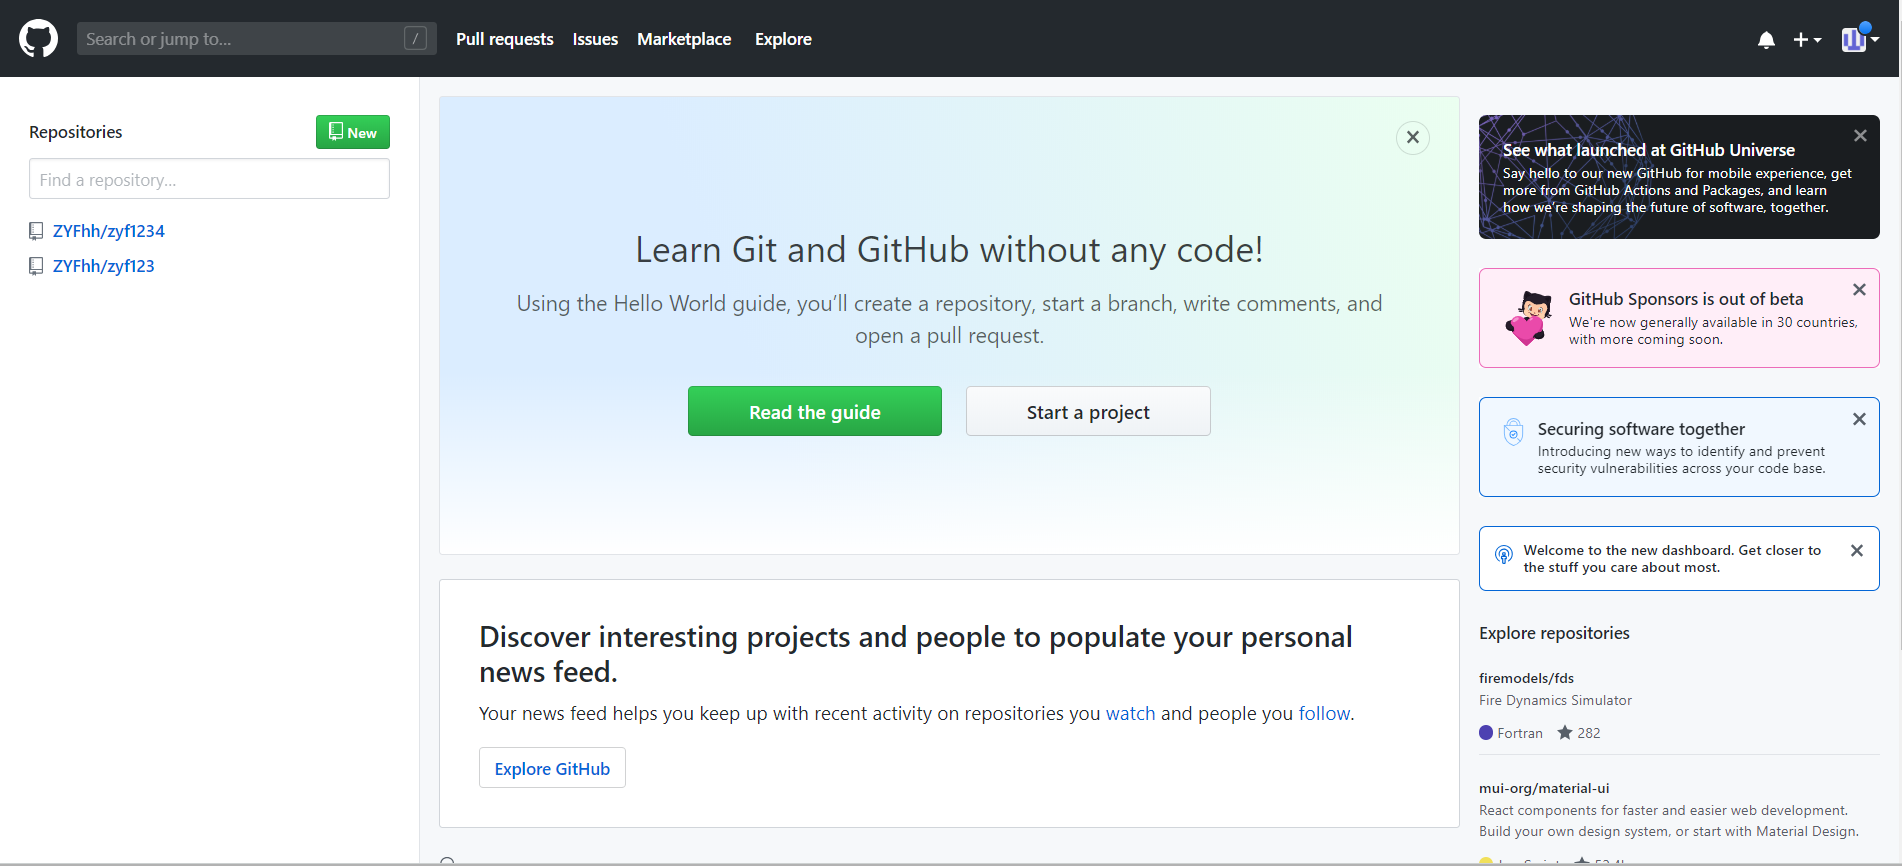
\includegraphics[scale=0.4]{github1.PNG}
	\caption{Github个人主页}
	\label{fig:gwrqc.jpg}
\end{figure}

\begin{figure}[h!]
	\centering
	
\includegraphics[scale=0.5]{github2.PNG}
	\caption{Github个人网站}
	\label{fig:ggrqc.jpg}
\end{figure}


\begin{figure}[h!]
	\centering
	
\includegraphics[scale=0.2]{guan.jpg}
	\caption{观察者截图}
	\label{fig:ggwqc.jpg}
\end{figure}

\begin{figure}[h!]
	\centering
	
\includegraphics[scale=0.2]{xue.jpg}
	\caption{学习强国截图}
	\label{fig:ggwrc.jpg}
\end{figure}

\begin{figure}[h!]
	\centering
	
\includegraphics[scale=0.2]{b.jpg}
	\caption{b站截图}
	\label{fig:ggwrqc.jpg}
\end{figure}

\begin{figure}[h!]
	\centering
	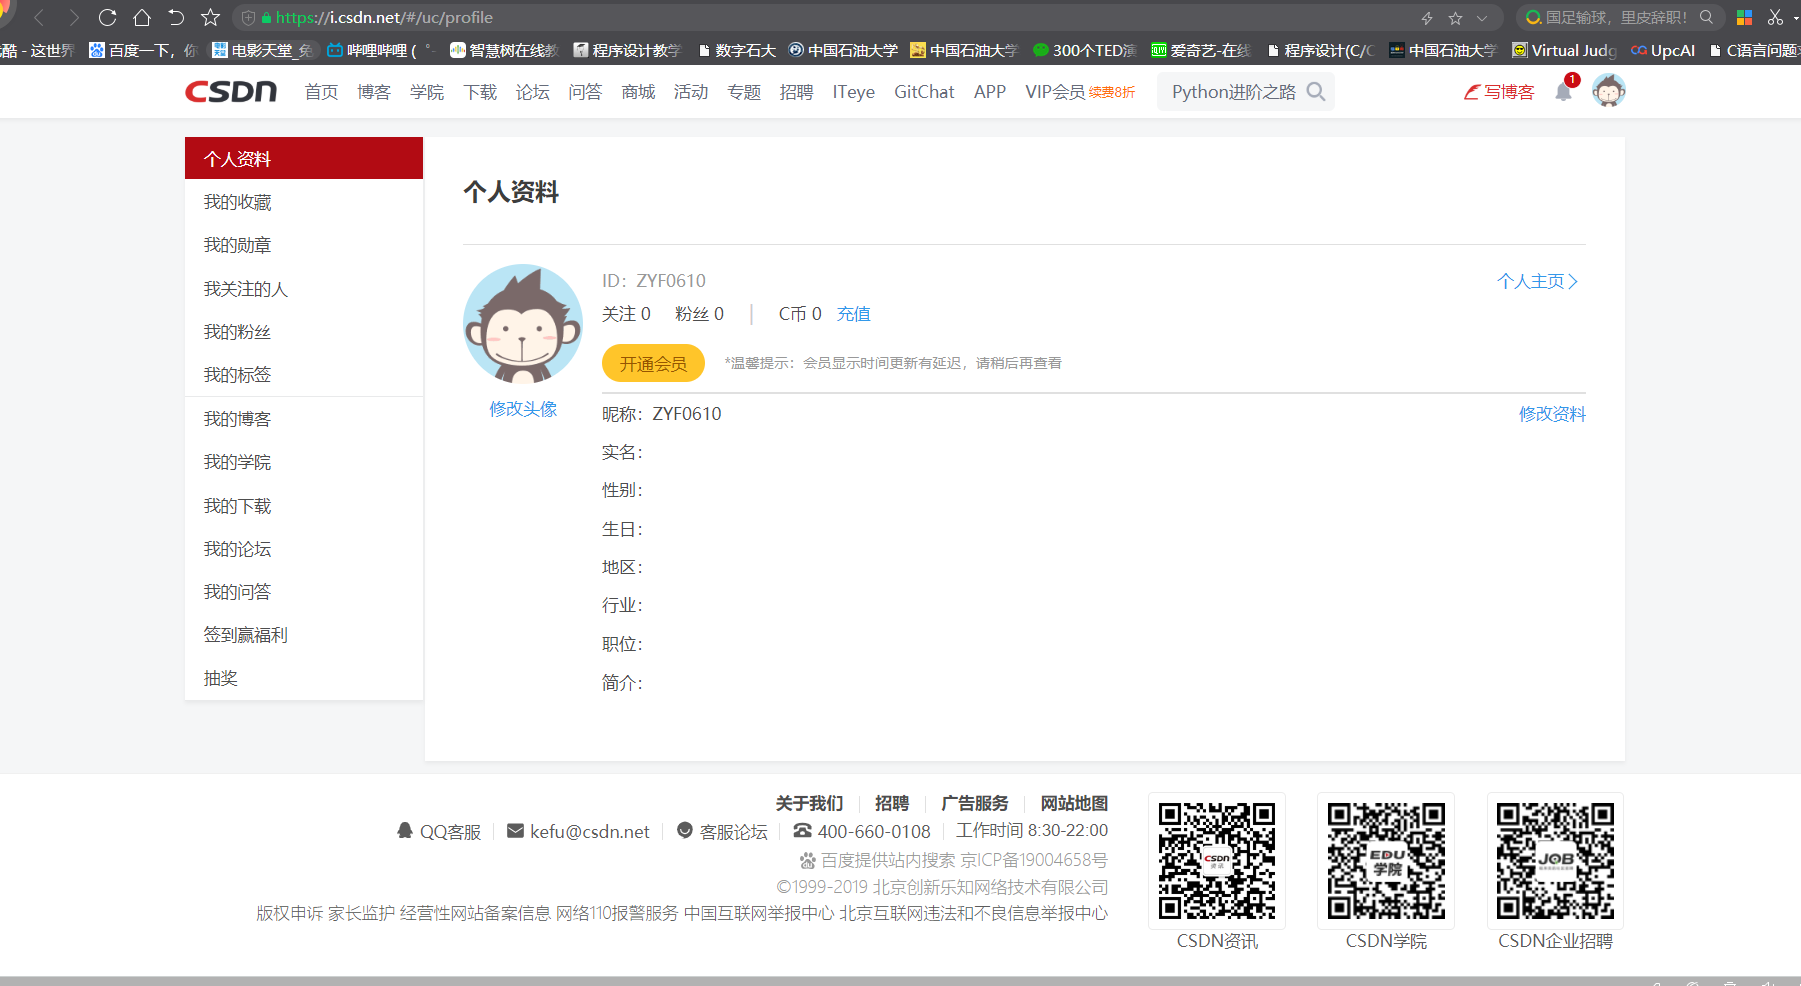
\includegraphics[scale=0.4]{CSDN.PNG}
	\caption{CSDN截图}
	\label{fig:ggwrq.jpg}
\end{figure}

\begin{figure}[h!]
	\centering
	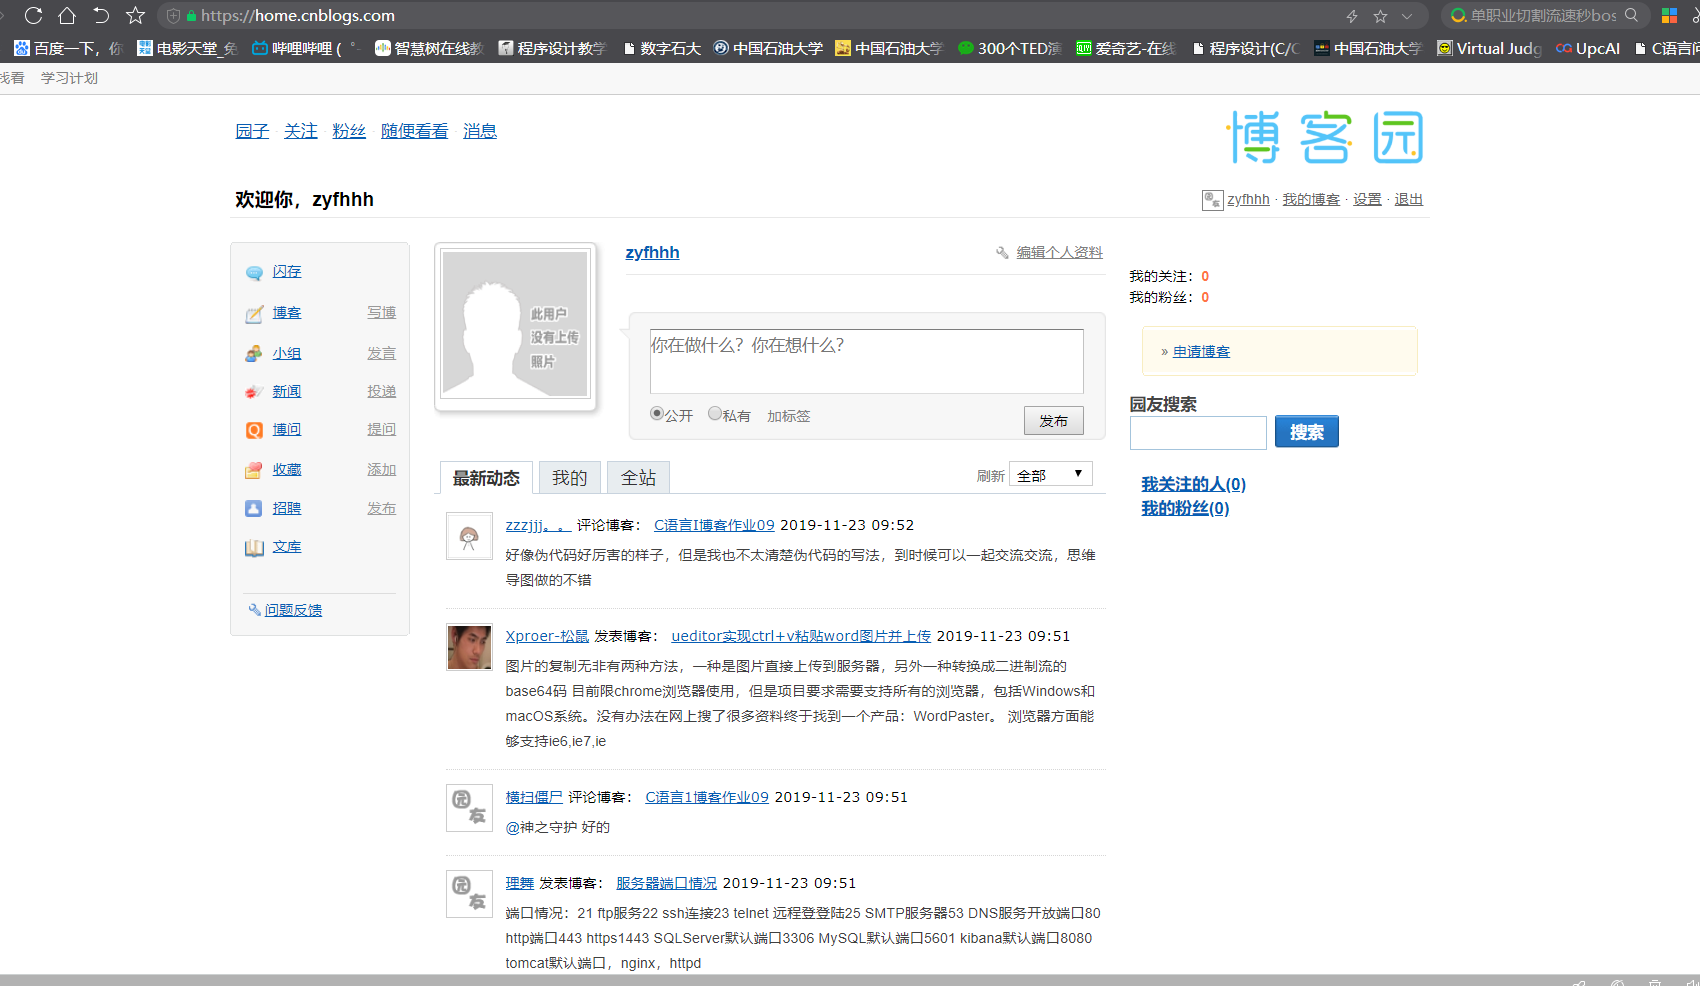
\includegraphics[scale=0.4]{boge.PNG}
	\caption{博客园截图}
	\label{fig:ggwrqgc.jpg}
\end{figure}

\begin{figure}[h!]
	\centering
	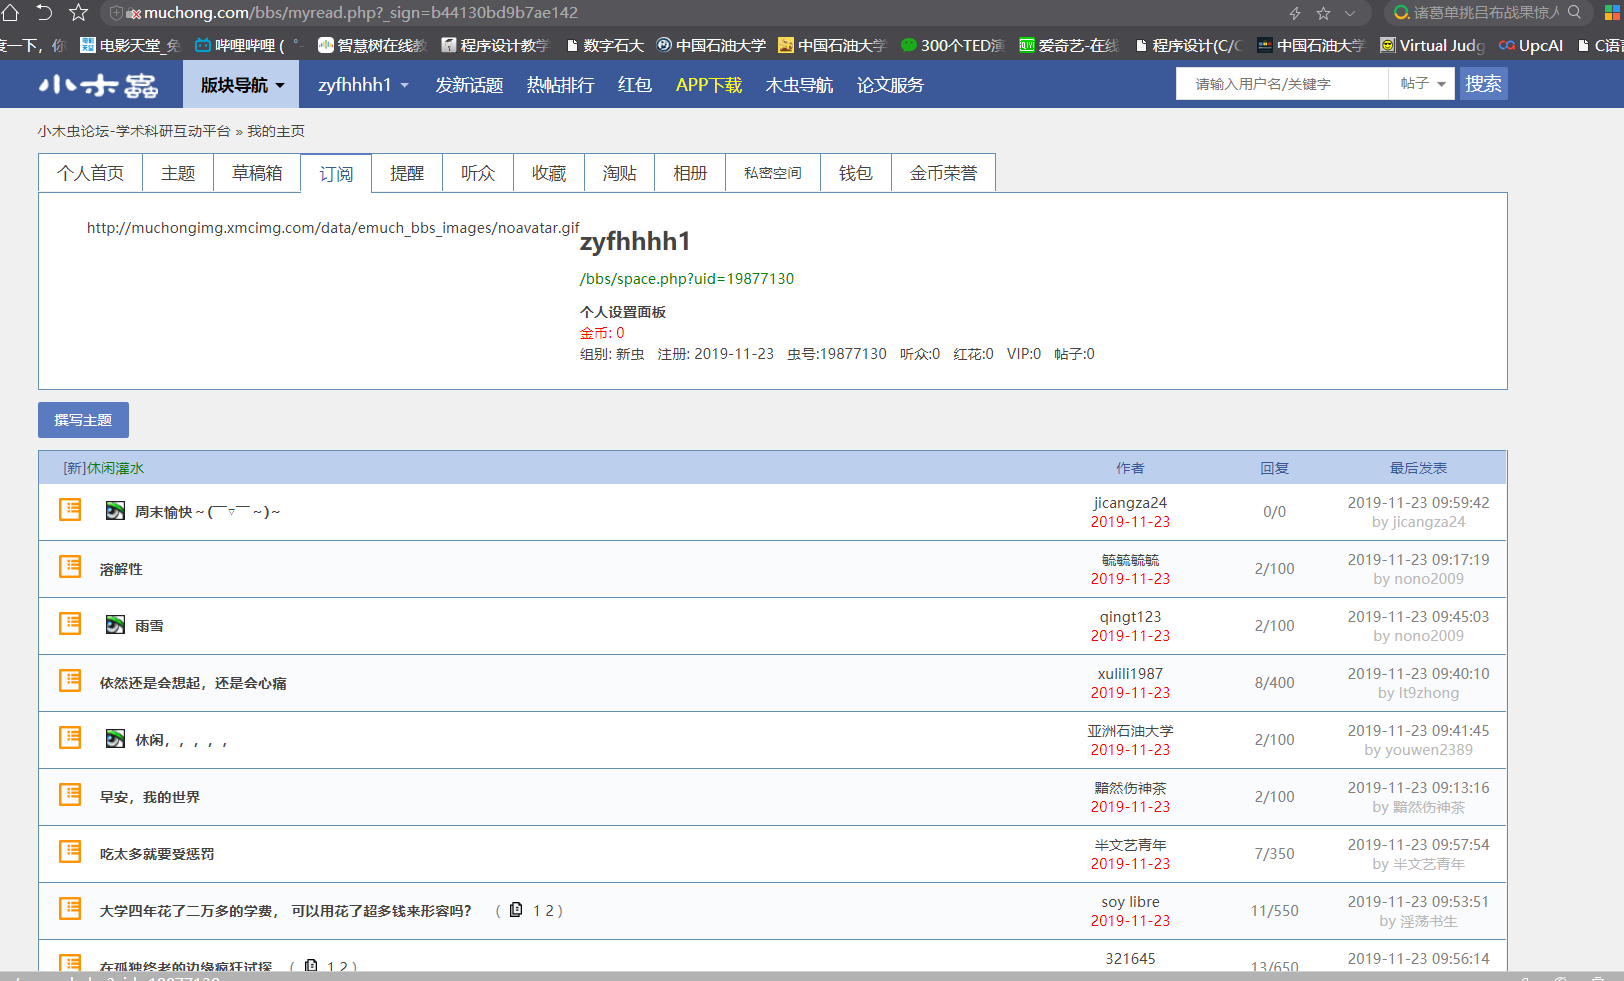
\includegraphics[scale=0.5]{bug.PNG}
	\caption{小木虫截图}
	\label{fig:ggwwrqc.jpg}
\end{figure}


\hspace*{\fill} \\


\bibliographystyle{plain}
\bibliography{references}


\end{document}
